% Plantilla Beamer para presentaciones de estudiantes de pregrado
% -------------------------------------------------------------
% Esta versión está rellena con datos de ejemplo ficticios.
% -------------------------------------------------------------

\documentclass[12pt]{beamer}

% Tema y colores
\usetheme{Madrid}
\usecolortheme{beaver}

% Paquetes básicos
\usepackage[utf8]{inputenc}
\usepackage[T1]{fontenc}
\usepackage[spanish]{babel}
\usepackage{lmodern}
\usepackage{graphicx}

\newcommand{\tituloTrabajo}{Análisis de Señales ECG}
\newcommand{\acronimoTrabajo}{ASECG-2025II} % Iniciales del trabajo-Periodo
\newcommand{\autorA}{Fulanito de Tal}
\newcommand{\autorB}{Sutanito de Tal}
\newcommand{\carrera}{Ingeniería Biomédica}
\newcommand{\codigoEstudianteA}{XXXXXXXX}
\newcommand{\codigoEstudianteB}{ MMMMMMMMMM}
\newcommand{\cursoCodigo}{SYSB - 2025II - A} % Acróinimo del curso - Periodo - Grupo. Ej: "SYSB - 2025II - A "
\newcommand{\cursoNombre}{Sistemas y Señales Biomédicas}
\newcommand{\docente}{Ing. Pablo Eduardo Caicedo-Rodríguez. Ph.D.}
\newcommand{\fechaEntrega}{\today}

% ----------------------------------
% Datos de la presentación (ejemplo)
\title[\acronimoTrabajo]{\tituloTrabajo}
\subtitle{\cursoNombre}
\author[\autorA \and \autorB]{\autorA \\\autorB}
\institute[]{\carrera\\Docente: \docente}
\date{\fechaEntrega}
% ----------------------------------

% Logo en todas las diapositivas (esquina inferior derecha)
\logo{
\includegraphics[height=1cm]{Escuela_Rosario_logo.            png}}

\begin{document}

% Portada
\begin{frame}[plain]
    \titlepage
\end{frame}

% Índice
\begin{frame}{Índice}
    \tableofcontents
\end{frame}

% Sección 1: Introducción
\section{Introducción}
\begin{frame}{Introducción}
    \begin{itemize}
        \item Motivación: Importancia del análisis EMG en rendimiento deportivo.
        \item Objetivos: Evaluar patrones de activación muscular.
        \item Estructura de la presentación.
    \end{itemize}
\end{frame}

% Sección 2: Metodología
\section{Metodología}
\begin{frame}{Metodología}
    \begin{enumerate}
        \item Selección de 20 voluntarios atletas.
        \item Adquisición de señales EMG con sensor MyoScan.
        \item Filtrado: Butterworth pasa-banda 20–450 Hz.
    \end{enumerate}
\end{frame}

% Sección 3: Resultados
\section{Resultados}
\begin{frame}{Resultados}
    \begin{figure}
        \centering
        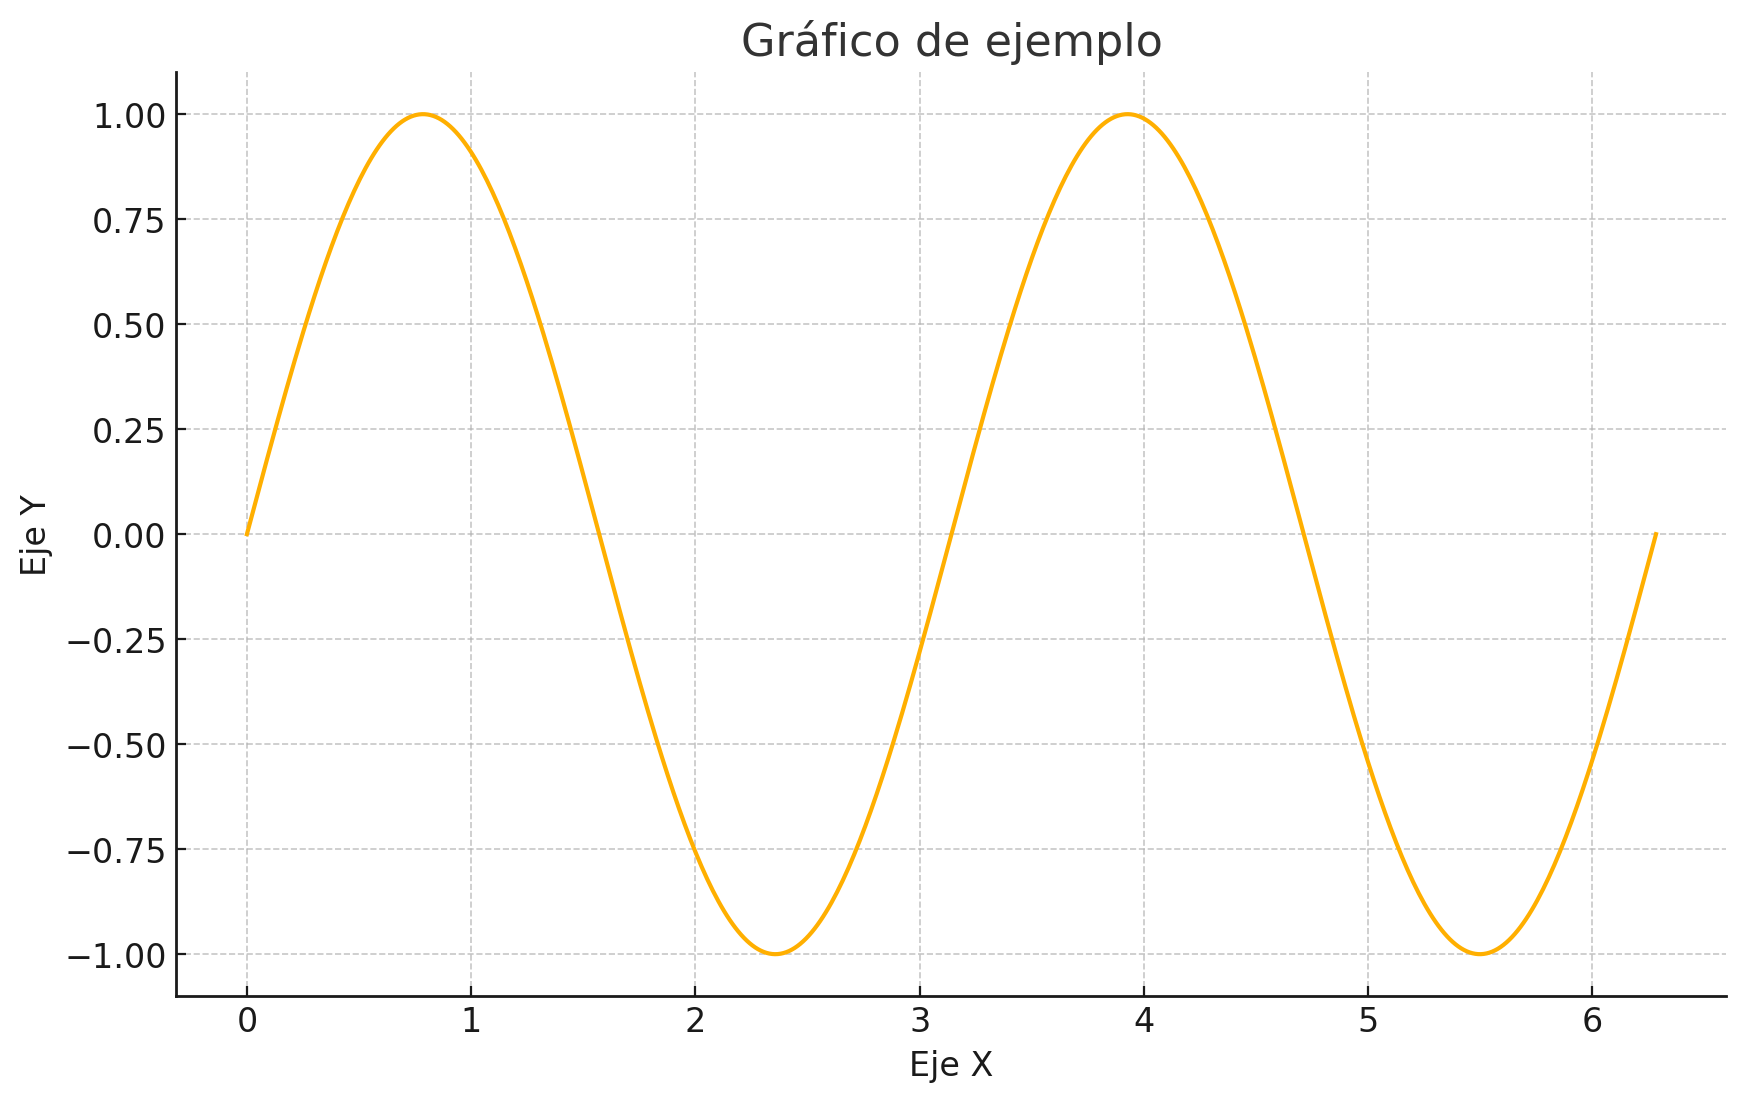
\includegraphics[width=0.7\textwidth]{ejemplo_grafico.png}
        \caption{Señal EMG promedio de cuádriceps durante ejercicio.}
    \end{figure}
\end{frame}

% Sección 4: Discusión
\section{Discusión}
\begin{frame}{Discusión}
    \begin{itemize}
        \item Aumento de amplitud refleja mayor reclutamiento.
        \item Comparación con estudios previos muestra consistencia.
    \end{itemize}
\end{frame}

% Sección 5: Conclusiones
\section{Conclusiones}
\begin{frame}{Conclusiones}
    \begin{itemize}
        \item La EMG es válida para monitoreo de rendimiento.
        \item Futuras líneas: integración con real-time biofeedback.
    \end{itemize}
\end{frame}

% Diapositiva final
\begin{frame}[plain]
    \centering
    \Huge ¡Gracias por su atención!\\[1cm]
    \small Preguntas y comentarios.
\end{frame}

\end{document}
